\documentclass[crop=false, class=book]{standalone}


%pacchetto per immagini
\usepackage{graphicx}

\usepackage[italian]{varioref}
\usepackage{copyrightbox}
\usepackage{url}

\begin{document}
	\section{Light estimation}
	Nel rendering in realtà aumentata è importante che gli oggetti virtuali siano il più possibile integrati con l'ambiente circostante. Una delle caratteristiche principali che permette all'occhio umano di percepire la posizione di un oggetto nello spazio è la luce, cioè il modo in cui esso viene illuminato e l'ombra che proietta. 
	Proprio per questo motivo, il framework ARCore mette a disposizione il \textit{Light estimation API}, che fornisce informazioni dettagliate riguardo l'illuminazione della scena, come spiegato nella documentazione ufficiale \cite{google2022light}.
	Tali informazioni sono necessarie per imitare i vari effetti che producono gli oggetti reali quando colpiti da una fonte di luce, che sono descritti dalla figura~\vref{fig:light_effects}:
	\begin{itemize}
		\item le \textbf{ombre} (\textit{shadows}), che sono direzionali e suggeriscono dove è collocata la fonte di luce;
		\item l'\textbf{ombreggiatura} (\textit{shading}), cioè l'intensità della luce che colpisce una certa faccia dell'oggetto;
		\item la \textbf{lumeggiatura} (\textit{specular highlight}), la macchia luminosa che compare su un oggetto lucido quando viene illuminato;
		\item la \textbf{riflessione} (\textit{reflection}), che può essere con proprietà speculari per oggetti completamente lucidi, come ad esempio uno specchio, oppure di diffusione, non dando un chiaro riflesso dell'ambiente circostante. 
	\end{itemize}
	
	\begin{figure}
		\centering
		\copyrightbox[l]{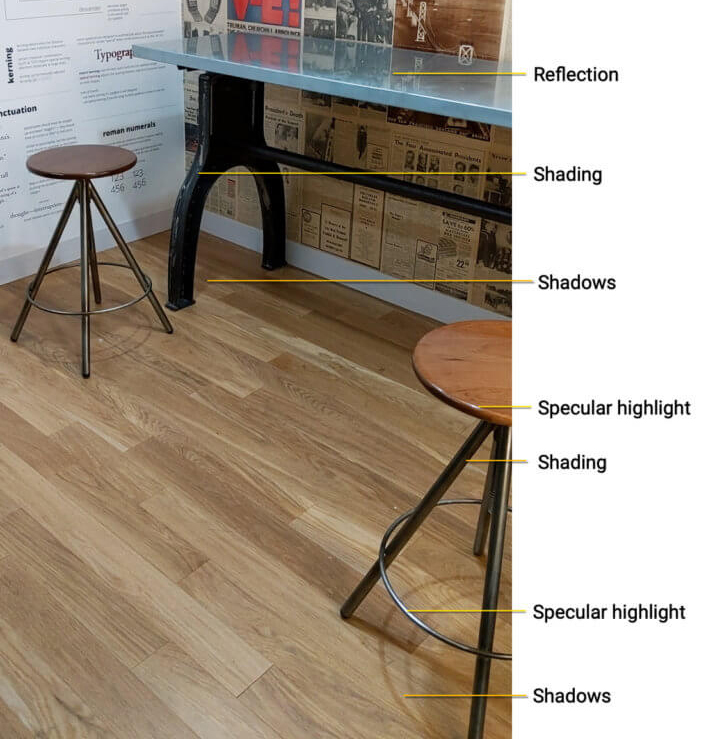
\includegraphics[width=0.5\textwidth]{./resources/images/light_estimation/light_effects}}%
			{Fonte: \url{https://developers.google.com}}
		\caption{Esempio degli effetti prodotti dagli oggetti quando sono illuminati.}
		\label{fig:light_effects}
	\end{figure}
    \noindent
	Le modalità per la gestione della stima della luce sono due, l'\textit{Environmental HDR mode} e l'\textit{Ambient intensity mode}. Durante la configurazione della sessione ARCore può essere scelta una delle due modalità, oppure disabilitare la stima della luce, come mostra il listing~\vref{lst:le_session} tratto dalla guida ufficiale.
	\\
	
	\begin{center}
		\begin{minipage}{0.95\textwidth}
			\begin{lstlisting}[caption={Configurazione della modalità di stima della luce.}, label={lst:le_session}, language=Kotlin]
			// Configura la sessione in modalità \verb|ENVIRONMENTAL_HDR|
			val config : Config = session.config
			config.lightEstimationMode = LightEstimationMode.ENVIRONMENTAL_HDR
			session.configure(config)
			
			// Configura la sessione in modalità \verb|AMBIENT_INTENSITY|
			val config : Config = session.config
			config.lightEstimationMode = LightEstimationMode.AMBIENT_INTENSITY
			session.configure(config)
				
			// Configura la sessione disabilitando la Light Estimation API
			val config : Config = session.config
			config.lightEstimationMode = LightEstimationMode.DISABLED
			session.configure(config)
			\end{lstlisting}
		\end{minipage}
	\end{center}


	

	\subsection{Environmental HDR mode}
		La modalità \textit{Environmental HDR} combina tre diverse API per replicare la luce reale, come descritti dalla figura~\vref{fig:env_HDR}.
	
		\paragraph*{Main Directional Light}
			Questa API calcola la direzione e l'intensità della fonte di luce principale, permettendo di posizionare correttamente l'ombra e la lumeggiatura dell'oggetto virtuale. Inoltre, questa funzionalità permette ad entrambi questi effetti ottici di venire corretti se cambia la posizione relativa dell'oggetto rispetto la fonte di luce
		
		\paragraph*{Ambient Spherical Harmonics}
			Questa funzionalità permette di rappresentare la luce ambientale della scena, parametrizzando l'intensità della luce proveniente dalle varie direzioni.
		
	
		\paragraph*{HDR Cubemap}
			Essa permette di riprodurre la riflessione di oggetti con superfici lucide. Tramite questa API viene modificata anche l'ombreggiatura e il colore dell'oggetto, che dipenderanno dalla tonalità dell'ambiente circostante.
	
		\begin{figure}
			\centering
			\copyrightbox[l]{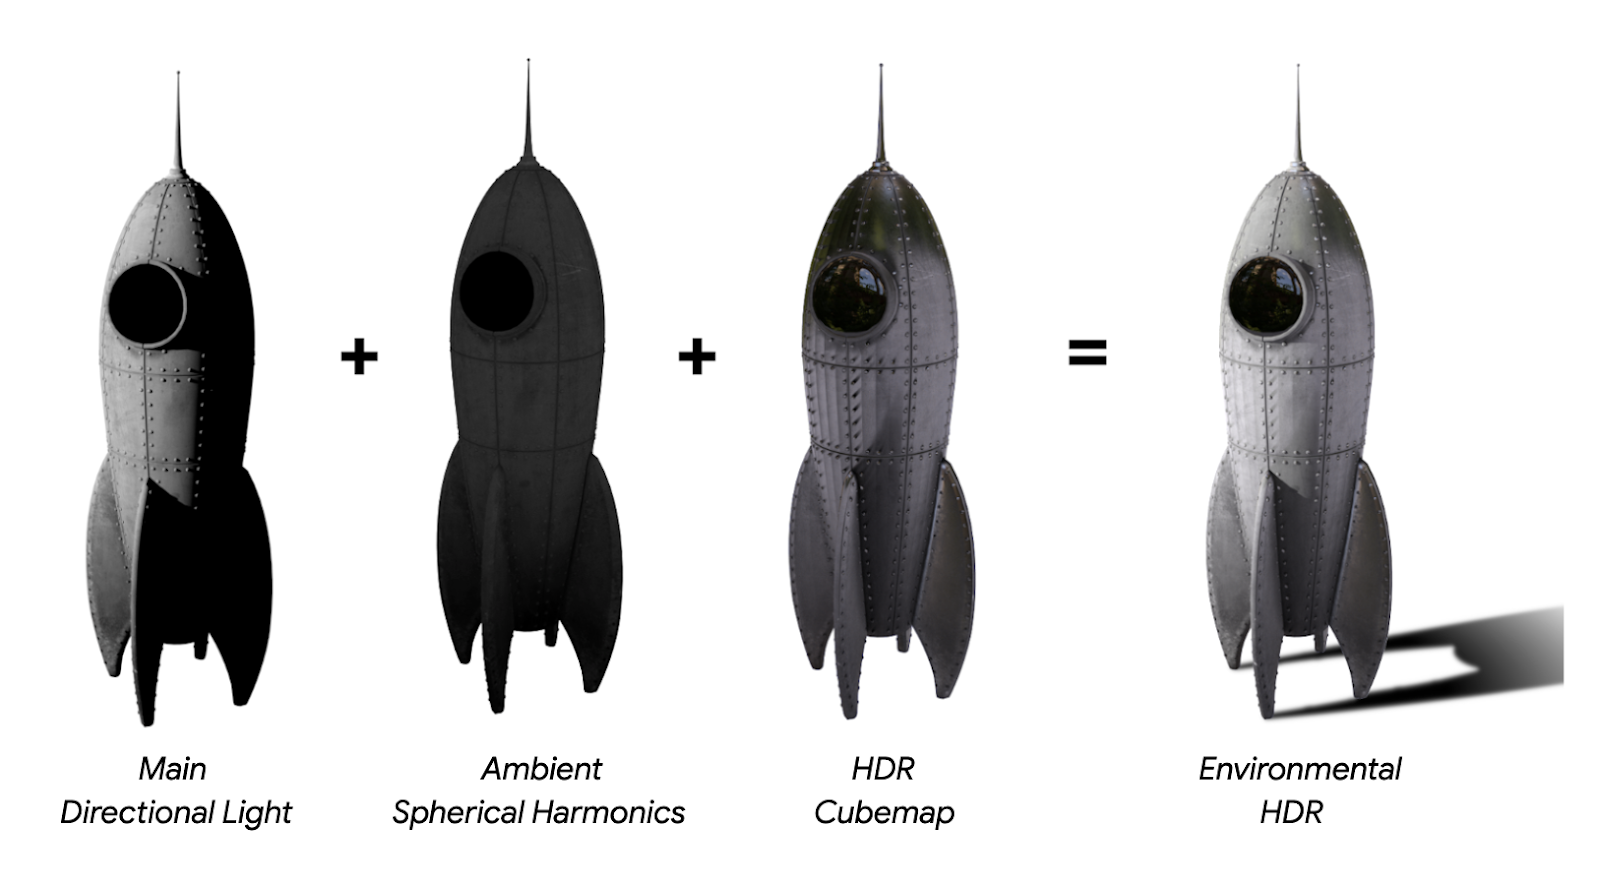
\includegraphics[width=0.8\textwidth]{./resources/images/light_estimation/env_HDR}}%
			{Fonte: \url{https://developers.googleblog.com}}
			\caption{Composizione della modalità Environmental HDR.}
			\label{fig:env_HDR}
		\end{figure}
	
	\subsection{Ambient intensity mode}
		La modalità \textit{Ambient intensity} determina l'intensità media dei pixel e la correzione del colore di una data immagine. Dopo aver filtrato l'intensità media di un insieme di pixel e il bilanciamento del bianco per ogni frame, vengono corretti la luce e il colore dell'oggetto virtuale, affinché si integri meglio con la scena \cite{suonsivu2020rgbd}. Questa modalità può essere utilizzata se la stima della luce non è critica, come per oggetti che possiedono già una propria illuminazione integrata.
	
	
\end{document}